\documentclass[ngerman]{article}

% Add all packages here
\usepackage[utf8]{inputenc}
\usepackage{amsmath, amsthm, amsfonts, amssymb}
\usepackage[margin=1in]{geometry}

% Useful custom commands I like. Feel free to send a PR :=)

% all number domains
\newcommand{\N}{\mathbb{N}}
\newcommand{\Z}{\mathbb{Z}}
\newcommand{\R}{\mathbb{R}}
\newcommand{\C}{\mathbb{C}}

% short versions of math arrows
\newcommand{\larr}{\leftarrow}
\newcommand{\rarr}{\rightarrow}
\newcommand{\lrarr}{\leftrightarrow}
\newcommand{\Larr}{\Leftarrow}
\newcommand{\Rarr}{\Rightarrow}
\newcommand{\Lrarr}{\Leftrightarrow}

% You can also just overshadow them by overwriting in the main.tex file
\title{Automatisierte Generation von Anki-basierten Karteikarten aus Markdownquellen}
\author{Lars Quentin\\Beteuung: Prof. Dr. Carsten Damm}
\date{03.03.2023}


\begin{document}
\maketitle
% ABSTRACT
\section*{Abstract}
Lorem ipsum dolor sit amet, consetetur sadipscing elitr, sed diam nonumy eirmod tempor invidunt ut labore et dolore magna aliquyam erat, sed diam voluptua. At vero eos et accusam et justo duo dolores et ea rebum. Stet clita kasd gubergren, no sea takimata sanctus est Lorem ipsum dolor sit amet. Lorem ipsum dolor sit amet, consetetur sadipscing elitr, sed diam nonumy eirmod tempor invidunt ut labore et dolore magna aliquyam erat, sed diam voluptua. At vero eos et accusam et justo duo dolores et ea rebum. Stet clita kasd gubergren, no sea takimata sanctus est Lorem ipsum dolor sit amet.
\tableofcontents
\newpage


\section{Einführung}
\subsection{Motivation}
Das Problem des Lernens, insbesondere in universitären Bereich, lässt sich in zwei distinkte Kategorien aufteilen: Das verständnisorienterte Lernen komplexer Themen und das faktenbasierte Lernen kleiner Details. Obwohl die meisten Klausuren eine Mischung aus den beiden Kategorien darstellen, erfordert jede Art unterschiedliche Vorgehensweisen:

\begin{itemize}
\item Im Falle verständnisbasierter komplexer Themen können Lernzettel geschrieben werden, indem Informationen zusammengefasst und umformuliert werden. Dies resultiert in immer noch großen komplexen Texten oder Stichpunktlisten, in welchen die einzelnen Informationen sehr nah miteinander verbunden sind. Die einzelnen Themen sind weniger isoliert, das erwartete Detailwissen ist geringer. Diese Klasse an Themen ist typisch für logisch-orientierte Studiengänge, wie z.B. Mathematik, Philosophie, Informatik oder Physik.
\item Im Gegensatz dazu erfordert das Lernen von faktenbasierten Details viel Auswendiglernen und wird meistens über Karteikarten praktiziert. Dieser Ansatz ist typisch für Studiengänge mit einem hohen Lernvolumen, wie z.B. Medizin, Biologie oder Sprachwissenschaften. Allgemein findet sich diese Problemart oft in komplexen, nicht-menschengemachten Systemen wieder.
\end{itemize}

Im digitalen Bereich gibt es für beide Arten von Klausurlernen kanonische Lösungen:
\begin{itemize}
  \item \textbf{Lernzettel:} Insbesondere in der Informatik wird für Lernzettel immer häufiger Markdown \cite{Markdown} verwendet. Markdown ist eine einfache, aber leistungsstarke Markup-Sprache, die einige Vorteile bietet: Zum einen kann sie ohne spezielle Software direkt von Menschen geschrieben werden, zum anderen ist sie einfach parsebar, wodurch sie mit vielen Tools genutzt werden kann. Zudem kann Markdown durch die simple, zeilenbasierte Struktur mit Git versioniert werden. Es unterstützt simple Medien wie Tabellen, Bilder und \LaTeX-Formeln, was es für die meisten Anwendungsfälle expressiv genug macht. Es gibt auch Tools wie Hedgedoc \cite{HedgeDoc} zum kollaborativen Live-Editieren, welches unter anderem auch als Instanz von der GWDG gehosted wird \cite{HedgeDocGWDG}. Es ist einfach, Markdown durch Applikationen wie Pandoc \cite{Pandoc} in HTML oder RevealJS-Presentationsfolien \cite{RevealJS} via Hedgedoc zu exportieren.
  \item \textbf{Karteikarten:} Digitale Karteikarten werden häufig mit sogenannten Spaced-Repitition Systemen (SRS) genutzt. Ein SRS ist ein Lernsystem, das Lernaufwand minimiert, indem es die Zeit zur nächsten Wiederholung der Frage auf Basis der bisherigen Kartenhistorie sowie der Selbsteinschätzung der Schwierigkeit anpasst. Das bedeutet, dass Fragen, die man leicht beantworten kann, seltener wiederholt werden als schwierigere Fragen, mit welchen man auch historisch bereits Probleme hatte.\\
    Das bei weitem beliebteste SRS ist Anki \cite{Anki}, ein Open-Source-Programm \cite{AnkiGithub}, das durch eine iOS-App \cite{AnkiiOS} finanziert wird. Es basiert auf Chromium \cite{QTWebEngine} und hat somit einen hohen Mediensupport. Anki bietet einen kostenlosen Cloud-Sync \cite{AnkiCloud}, der es ermöglicht, Karteikarten auf verschiedenen Geräten zu synchronisieren. Darüber hinaus gibt es eine kostenlose, von der Community erstellte Androidversion. Anki hat auch eine große Bibliothek von Decks, die von der Community geteilt werden, sowie PlugIns-Support \cite{AnkiPlugins}, die es Benutzern ermöglicht, die Funktionalität von Anki zu erweitern.
\end{itemize}

Trotz der Vorteile, die sowohl Lernzettel als auch Karteikarten bieten, haben sie auch ihre Nachteile. Lernzettel sind ineffizient, wenn es darum geht, Details zu lernen, da sie oft sehr verbos sind und eine geringere Informationsdichte haben. Darüber hinaus kann man keinen expliziten Fokus auf Themen setzen, welche einem besonders schwerfallen, da der Text sich nicht so einfach in atomare Fakten aufteilen lässt. Auf der anderen Seite verlieren Karteikarten schnell ihre Reihenfolge. Zuletzt kann man zwischen Karteikarten keinen Kontext erhalten, welcher gegebenenfalls benötigt wird um das größere Konzept zu verstehen.

\newpage

In diesem Praktikumsbericht wird eine Lösung vorgestellt, Lernzettel mit Markdown und und Karteikarten mit Anki logisch zu verbinden. Die Idee basiert auf dem Konzept von literate Programming.\\

Literate Programming ist ein Konzept, das von Donald E. Knuth entwickelt wurde \cite{LitProg}. Es kombiniert Programmcode mit der Dokumentation, so dass der Code und die Dokumentation in einer Datei vereint werden. Die Funktionen sind innerhalb der Dokumentation integriert und die gesamte Dokumentation lässt sich ausführen. Das ursprüngliche Konzept von Literate Programming verwendet eine eigene Sprache namens "WEB", die von Knuth entwickelt wurde. WEB-Quelldateien kompilierten entwedr zu Pascal oder zu \TeX \cite{WebIntroduction}.\\

Moderne Umsetzungen von Literate Programming sind Jupyter Notebooks \cite{Jupyter}. Jupyter Notebooks sind interaktive Dokumente, die Code, Markdowntext und Medien durch sogenannte Zellen in einem Dokument vereinigen. Da Jupyter Notebooks ohne explizite Programmierumgebung gehosted in einem Webbrowser, zum Beispiel via GWDG Jupyter Hub \cite{JupyterGWDG} oder Google Colab \cite{Colab}, benutzbar sind haben sie eine geringe Einstiegshürde. Hierdurch sind sie interdisziplinär in der Forschung omnipräsent. Sie implementieren das Konzept von Literate Programming, indem man den Code als Teil des Dokumentes betrachtet statt als isolierte Einheit.

\subsection{Ziele und Beitr\"age}
Das Ziel dieser Arbeit ist, analog zum Konzept des literate Programmings, Karteikarten in Markdownzusammenfassungen zu integrieren. Hierdurch wird es möglich, das gesamte Markdown-Ökosystem zum Erstellen, Bearbeiten und Versionieren der Karteikarten zu nutzen. Einerseits ermöglicht dies, dass Karteikarten den Kontext und die Reihenfolge behalten, welche für das Lernen komplexer Themen erforderlich ist. Andererseits soll ein automatischer Anki-Export erstellt werden, der die Nutzung von Spaced Repitition für ein effizienteres Lernen von Fakten ermöglicht.\\

Im Rahmen dieses Praktikums wurden mehrere Beiträge geleistet, um die gesteckten Ziele zu erreichen. Zunächst wurde ein neuer Dateistandard für \texttt{.anki.md} Dateien entwickelt, um die Integration von Karteikarten in Markdownzusammenfassungen zu ermöglichen.

Darüber hinaus wurde ein Tool erstellt, das automatisch aus einem Ordner mit Markdown-Dateien ein Ankideck erstellen kann \cite{Ankiding}. Hierbei wird die Ordnerstruktur auf die Struktur der Ankidecks übertragen, und es wird sämtliche Markdown Syntax sowie das Rendering von \LaTeX-Formeln unterstützt. Das Tool kann auch mit der Mobilversion von Anki genutzt werden. Zudem kann mit dem Ankideck offline gelernt werden, da alle verlinkten Bilder in das Deckarchiv gespeichert werden. Weitere Features wie ein Darkmode wurden ebenfalls implementiert.\\

Zuletzt wurden Git-Repository-Templates für GitLab \cite{GitlabTemplate} und GitHub \cite{GithubTemplate} konzipiert und erstellt, mit denen automatisch via Continuous Integration nach jedem Commit ein aktualisiertes Ankideckarchiv erstellt wird. Dies ermöglicht die Erstellung von Ankikarten ohne Installation von Software oder technischem Verständnis des Konvertierungsprozesses.

\newpage


\section{Softwarekonzeptionierung und Methodologie}
\subsection{Entwurf einer Markdownerweiterung}
Markdown ist zwar sehr verbreitet, jedoch gibt es keine universale Markdownspezifikation. Stattdessen gibt es viele verschiedene Varianten, welche leicht aber inkompatibel voneinander abweichen. Somit, bevor man den Markdownstandard erweitern kann, muss ein Markdownstandard spezifiziert werden.

Für den Anwendungsfall dieses Praktikums wird als Basis der am weitesten verbreite CommonMark \cite{CommonMark} Standard genommen. Dieser ist sehr simpel, jedoch von den meisten Implementationen unterstützt. Insbesondere ist er zu den meisten größeren Standards kompatibel.

Desweiteren soll der hier entwickelte Karteikarten-Standard auch mit folgenden Markdownstandards kompatibel sein:
\begin{itemize}
  \item \textbf{GitHub Flavored Markdown (GFM) \cite{GFM}:} Benötigt für die automatische Kartengenerierung über Githubrepositories.
  \item \textbf{GitLab Flavored Markdown (GLFM) \cite{GLFM} :} Benötigt für die automatische Kartengenerierung über Gitlabrepositories.
  \item \textbf{HedgeDoc Flavored Markdown 2.0 (HFM 2.0) \cite{HFM2}:} Benötigt zum kollaborativen Erstellen von Karteikarten über die Hedgedoc-Infrastruktur der GWDG \cite{HedgeDocGWDG}.
\end{itemize}

Somit, aufbauend auf CommonMark, wird im Rahmen dieses Praktikums ein Standard für \texttt{.anki.md}-Dateien definiert. Der Standard hat folgende Ziele:
\begin{itemize}
  \item Eindeutige Parsebarkeit
  \item Renderunterstützung in GitHub, GitLab sowie HedgeDoc
  \item Einfache Syntax, welche sich manuell mit wenig Extraaufwand schreiben lässt
  \item Gute Lesbarkeit in Codeform
  \item Keine Kollisionen mit normalem Text; keine falschen positiven Erkennungen
\end{itemize}

Die unsterstützte Karteikartensyntax funktioniert wiefolgt:
\begin{figure}[H]
\centering
\begin{lstlisting}
> Q: Dies ist eine Frage
>
> Sie kann ueber mehrere Zeilen gehen
>
> A: Das ist die Antwort
>
> Auch hier kann man mehrere Zeilen haben
>
> Oder **sogar** die komplette Markdownsyntax nutzen
\end{lstlisting}
  \caption{Ein Beispiel der genutzten Karteikartensyntax}
\end{figure}
In den verschiedenen Umgebungen sieht es wiefolgt aus:

\begin{figure}[H]
\centering
\begin{tabular}{ccc}
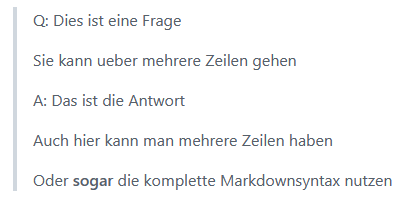
\includegraphics[width=50mm]{./figures/GH_Syntax1} & 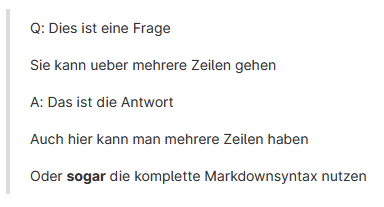
\includegraphics[width=50mm]{./figures/GL_Syntax1} & 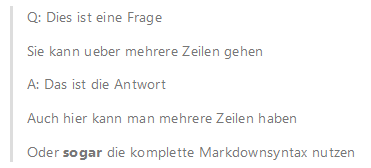
\includegraphics[width=50mm]{./figures/HD_Syntax1} \\
GitHub & GitLab & HedgeDoc \\
\end{tabular}
\caption{Rendering der in Abb. 1 definierten Syntax}
\end{figure}

Als Alternativansätze wurden folgende Syntaxmöglichkeiten betrachtet:

\paragraph{Durch Horizontallinien getrennte Karteikartenseiten:}~\\
Diese Syntax würde wiefolgt aussehen:
\begin{figure}[H]
\centering
\begin{lstlisting}
---
Q: Dies ist eine Frage

Sie kann ueber mehrere Zeilen gehen
---
A: Das ist eine Antwort

Auch hier kann man mehrere Zeilen haben

Oder **sogar** die komplette Markdownsyntax nutzen
---
\end{lstlisting}
  \caption{Ein Beispiel einer alternativen Karteikartensyntax}
\end{figure}

Während diese Syntax sehr leserlich in Markdownform sowie sehr einfach zu schreiben ist, hat sie mehrere Probleme.

Zu aller erst kann diese Syntax nicht in der ersten Zeile benutzt werden, da es dann Kollisionen mit dem sogenannten Front Matter gibt; ein auf YAML basierendes Metadatenformat innerhalb der Markdowndatei. Front Matter wird sowohl von GFM, GLFM als auch HFM unterstützt.\\

Zudem ist es sehr einfach syntaktische Fehler zu machen, da es sehr einfach passieren kann die letzte horizontale Linie zu setzen.\\

Zuletzt ist das visuelle Rendering sehr unintuitiv, insbesondere da ohne freie Zeile die horizontale Linie in eine Überschrift umgewandelt wird

\begin{figure}[H]
\centering
\begin{tabular}{ccc}

\includegraphics[width=50mm]{./figures/GH_Syntax2} & 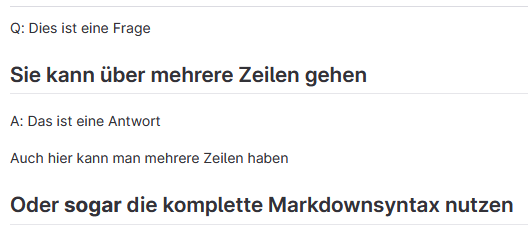
\includegraphics[width=50mm]{./figures/GL_Syntax2} & 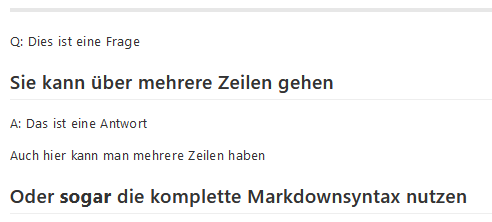
\includegraphics[width=50mm]{./figures/HD_Syntax2} \\
GitHub & GitLab & HedgeDoc \\
\end{tabular}
\caption{Rendering der in Abb. 3 definierten Syntax}
\end{figure}

\paragraph{Karteikarten in Tabellenform:}~\\
Diese Syntax würde wiefolgt aussehen:
\begin{figure}[H]
%\centering
  \begin{lstlisting}
| Question                       | Answer                              |
| ------------------------------ | ------------------------------------|
| Wofuer steht DFA?              | Deterministischer endlicher Automat |
| Welche Laufzeit hat Quicksort durchschnittlich? | O(n log n)         |
\end{lstlisting}
  \caption{Beispiel für eine tabellenbasierte Karteikartensyntax}
\end{figure}

Diese Syntax sieht gerendert sehr schön aus.

\begin{figure}[H]
\centering
\begin{tabular}{ccc}
  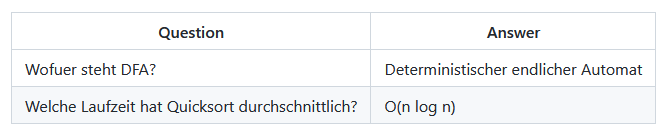
\includegraphics[width=0.5\textwidth]{./figures/GH_Syntax3} &
  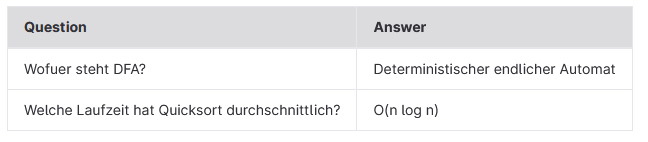
\includegraphics[width=0.5\textwidth]{./figures/GL_Syntax3}\\
GitHub & GitLab\\
\end{tabular}
  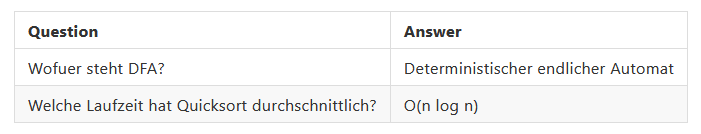
\includegraphics[width=0.5\textwidth]{./figures/HD_Syntax3} \\
  HedgeDoc
\caption{Rendering der in Abb. 5 definierten Syntax}
\end{figure}

Jedoch hat auch diese Syntax mehrere Nachteile. Zu aller erst eignet sich diese Syntax nicht für die Anwendung durch literate Programming, da hierdurch nur viele einzeilige Tabellen zwischen dem Text entstehen würden. Zudem ist diese Art von Syntax sehr aufwändig für den Endnutzer, sofern dieser kein WYSIWYG-Editor nutzt. Zuletzt ist eine Zelle viel zu restriktiv. Es ist weder möglich, eine Antwort über mehrere Zeilen zu definieren, noch ist es möglich sinnvoll Bilder einzubinden.

\paragraph{Karteikarten durch XML Objekte:}~\\
Diese Syntax würde wiefolgt aussehen:
\begin{figure}[H]
\centering
\begin{lstlisting}
<anki>
  <q>
    Dies ist eine Frage

    Sie kann ueber mehrere Zeilen gehen
  </q>
  <a>
    Dies ist die Antwort

    Auch hier kann man mehrere Zeilen haben

    Oder sogar die komplette Markdownsyntax nutzen
  </a>
</anki>
\end{lstlisting}
  \caption{Beispiel für eine XML-basierte Karteikartensyntax}
\end{figure}

Der Inhalt hiervon wird leider von Github gar nicht gerendered, weswegen es für unseren Anwendungsfall nicht nutzbar ist. In GitLab sowie HedgeDoc werden die Tags auch nicht angezeigt, jedoch ist zumindest der Inhalt noch sichtbar.

\subsection{Unterst\"utzung von \LaTeX-Formeln}
Die Desktopversion von Anki ermöglicht bereits die Darstellung von \LaTeX-Formeln auf Karteikarten. Dabei wird beim ersten Anzeigen einer Karteikarte ein Bild der Formel mit einer lokal installierten \LaTeX-Engine gerendert und in der Anki-eigenen Mediendatenbank gespeichert. Die Formel in der Karteikarte wird durch das gerenderte Bild ersetzt. Somit muss jede Formel nur einmal gerendert werden.Insbesondere wird die Mediendatenbank über die Cloud synchronisiert. Somit reicht es, dass das erste Gerät eine \LaTeX-Intallation hat.\\

Die Mobilappliaktionen wie AnkiDroid oder die iOS-Version haben jedoch keine Unterstützung für \LaTeX. Dies stellt normalerweise kein Problem dar, da bei der Karteikartenerstellung über die Desktopapplikation bereits die Formel gerendered wird. Da der Karteikartengenerator hier jedoch eigenständig zu Anki funktioniert, muss in Rahmen dieser Applikation auch die Formelgeneration übernommen werden.\\

Die Formelumwandlung ist jedoch nicht trivial. Das Problem hierbei sind die unterstützten Ausgabeformate:
\begin{itemize}
  \item \textbf{Portable Document Format (PDF):} PDF ist ein sehr komplexes Dateiformat. Es hat viele, sehr umfangreiche Standards und wird von nur wenig Applikationen korrekt implementiert. Somit ist die Rasterisierung von PDF von Applikationen, welche nicht von Adobe hergestellt wurden, sehr fehleranfällig.
  \item \textbf{Device independent file format (DVI):} DVI ist ein selten genutztes, obskures Seitenformat. \LaTeX ist die einzige große Applikation, welche noch DVI als Ausgabeformat unterstützt, da Knuth es als formell unterstütztes Ausgabeformat von \TeX definierte. Dementsprechend wenig Applikationen unterstützen DVI.
  \item \textbf{Encapsulated PostScript (EPS):} EPS ist ein für Drucker entwickeltes Vektorgrafikformat. Somit unterscheidet es sich sowohl von der Funktionalität als auch von der Nutzerschaft stark von pixelbasierten Bildformaten wie PNG.
\end{itemize}

Im folgenden wird eine Taxonomie der Konvertierungmöglichkeiten vorgestellt:
% TODO: Citations.
\begin{itemize}
  \item \textbf{ImageMagick:} ImageMagick \cite{ImageMagick} ist ein open-source Programm zur Bearbeitung von Raster- und Lektorgrafiken. Diese Lösung ist auch die etablierte Lösung des \TeX-Stackexchange \cite{TeXStackexchange}. Sie ist simpel, hat jedoch zwei große Nachteile. Einerseits benötigt man sowohl \LaTeX als auch ImageMagick als externe Abhängigkeit; andererseits benötigt sie manuelle Anpassungen der Sicherheitsrichtlinien, was root vorraussetzt.
  \item \textbf{PDFium:} PDFium \cite{PDFium} ist die C++ PDF Bibliothek welche von Chromium \cite{Chromium} benutzt wird. Da man zum kompilieren jedoch den kompletten Chromium-Browser kompilieren muss, ist der Aufwand zu hoch. Chromium braucht mindestens 8GB RAM sowie 100GB Festplattenspeicher zur Kompilation und braucht auf älterer Hardware mehrere Stunden.
  \item \textbf{KaTeX:} KaTeX \cite{KaTeX} ist eine in Javascript geschriebene \LaTeX-Implementation, welche auf Webseiten eingebunden werden kann um Formeln darzustellen. Sie wird unter anderem auch von GitHub und GitLab genutzt. Jedoch würde dies eine LaTeX-Engine wie Deno \cite{Deno} oder Node.js \cite{Node} vorraussetzen, welche sehr komplex einzubinden wäre.
  \item \textbf{dvisvgm:} Zuletzt gibt es \texttt{dvisvgm} \cite{dvisvgm}, welches PDF, DVI und EPS-Dokumente in SVG-Vektorgrafiken umwandeln kann. SVG ist das häufigst genutzte Vektorgrafikformat, für welches viele PNG
    Konvertierungsmöglichkeiten existieren.
\end{itemize}

In unserem Fall haben wir uns für \texttt{dvisvgm} entschieden. Es ist eine kleine Laufzeitabhängigkeit, ist jedoch in jeder kompletten TeXLive- sowie MikTeX-Installation vorhanden. Dies bedeutet, dass wir keine Abhängigkeiten haben, welche nicht auch von Anki vorrausgesetzt werden. Die von \texttt{dvisvgm} erstellen SVG-Grafiken werden dann durch \texttt{resvg} \cite{resvg} zu PNG exportiert.

\subsection{Commitbasierte Kartengeneration durch Continuous Integration (CI)}
Im Rahmen der Continuous Integration (CI) Softwarepraktik bieten alle großen Git-Repository-Hostinganbieter sogenannte Workflows an. Hierbei wird zu spezifischen Events wie Commits oder Pull Requests ein Container ausgeführt, welcher automatisiert Aufgaben erfüllen kann. Unter den typischen Aufgaben von CI zählen das Analysieren von Source Code nach Best Practises, dem sogenannten linting, der Ausführung automatisierter Tests sowie der Erstellung von Kompilaten.\\

In unserem Fall ermöglichen wir durch die Nutzung von CI-Workflows eine automatische Erstellung von Ankidecks aus Gitrepositories. Dieser Anwendungszweck ist so gedacht, dass die Nutzerschaft gemeinsam kollaborativ via Git eine Ordnerstruktur an Anki-Markdowndokumenten erstellt. Im Rahmen dieses Praktikums wurden sowohl für GitLab \cite{GitlabTemplate} als auch für GitHub \cite{GithubTemplate} Repositoryvorlagen erstellt. Im folgenden wird ohne Beschränkung der Allgemeinheit die Funktionsweise anhand von Gitlab vorgestellt:

\begin{enumerate}
  \item Ein Nutzer macht eine Änderung an dem Repository und pusht den Commit auf den GitLab-Server. Die GitLab-Instanz startet einen OCI-Ubuntucontainer welcher das Repository im current working directory (CWD) eingebunden hat.
  \item Das System wird via \texttt{apt} aktualisiert und es werden folgende Abhängigkeiten installiert:
    \begin{itemize}
      \item curl (Zur Installation von Rust via \texttt{rustup} benötigt)
      \item git (Für den Download des Konvertierungsprogramms benötigt)
      \item \LaTeX (Zur Darstellung von Formeln zur Laufzeit benötigt)
      \item C-Compiler via \texttt{build-essential} (Zur Kompilation benötigt)
      \item pkg-config (Zur Kompilation benötigt)
      \item OpenSSL (Zur Kompilation benötigt)
      \item Rust-Compiler (Zur Kompilation benötigt)
    \end{itemize}
  \item Das Konvertierungsprogramm wird in das CWD via git gecloned und kompiliert.
  \item Das kompilierte Programm wird auf den Ordner mit den Anki-Markdowndokumenten angewandt.
  \item Das resultierende Karteikartenarchiv wird als Artifact den Nutzern bereitgestellt.
\end{enumerate}

\section{Implementation}
\subsection{Offlineunterst\"utzung}
\subsection{\LaTeX-Unterst\"utzung}
\section{Diskussion}
\subsection{Audio- und Videounterst\"utzung}
\subsection{Geplante Weiterentwicklung und Einsatz der Software}
\newpage
\section{Literaturverzeichnis}
\printbibliography
\end{document}
